\section{The De-Noising Effect of Multi-Task Learning}


In this part, we shall establish the intuition that adding more data helps in multi-task learning by reducing the variance of the estimator.
We achieve this through tight generalization bounds obtained from random matrix theory.
We focus the case of two tasks to provide a complete picture on how covariate and model shifts can affect the type of transfer.

Recall that the test error of $\hat{\beta}_{t}^{\MTL}$ consists of two parts
\begin{align}
	\te(\hat{\beta}_t^{\MTL}) = \hat{w}^2 \bignorm{\Sigma_2^{1/2} (\hat{w}^2 X_1^{\top}X_1 + X_2^{\top}X_2)^{-1}X_1^{\top}X_1 (\beta_s - \hat{w}\beta_t)}^2 + \sigma^2\cdot \bigtr{(\hat{w}^2 X_1^{\top}X_1 + X_2^{\top}X_2)^{-1}\Sigma_2}. \label{eq_te_model_shift}
\end{align}
It is not hard to show that the variance of $\hat{\beta}_t^{\MTL}$ is reduced compared to $\hat{\beta}_t^{\STL}$ (following the argument of Proposition \ref{prop_monotone}), i.e.
\[ \sigma^2\cdot \bigtr{(\hat{w}^2 X_1^{\top}X_1 + X_2^{\top}X_2)^{-1}\Sigma_2} \le \sigma^2\cdot \bigtr{(X_2^{\top}X_2)^{-1}\Sigma_2}. \]
Because of model shift however, i.e. $\beta_s \neq \beta_t$.
We can no longer guarantee that $\te(\hat{\beta}_{t}^{\MTL}) \le \te(\hat{\beta}_t^{\STL})$.
The main result of this part show deterministic conditions under which we get positive or negative transfer.
And the conditions depend only on the covariate shift matrix $M$, the difference of the task models, and the number of per-task data points.
In order to characterize $\te(\hat{\beta}_t^{\MTL})$ and $\te(\hat{\beta}_t^{\STL})$, the technical crux of our approach relies on deriving the limit of the trace of matrix inverse in the high-dimensional setting.
To illustrate the idea, we observe that by using Lemma \ref{lem_minv}, we have that
\[ \te(\hat{\beta}_t^{\STL}) = \frac{\sigma^2}{n_2 - p}\bigtr{\Sigma_2^{-1}}. \]
We shall also derive the limit of $\te(\hat{\beta}_t^{\MTL})$.
\todo{write a brief technical overview}

%In this case, $\beta_s$ and $\beta_t$ are different.
%, or implicitly add a regularization on $B$.
%\todo{We focus on the former case in this section.}
%, we consider the case when $r=1$ since there are only two tasks.
%We begin by considering the simplified equation \eqref{eq_mtl_basic} to solve for the target task.
%This is equivalent to setting $W_i = 1$ for the two tasks in equation \eqref{eq_mtl}.
%The result of this simplified setting will set up the ground for solving equation \eqref{eq_mtl} when we also optimize $W_1$ and $W_2$.
%By putting the two tasks together, we get
%\begin{align*}
%	\hat{\beta}_{s,t} &= (X_1^{\top}X_1 + X_2^{\top}X_2)^{-1} (X_1^{\top}Y_1 + X_2^{\top}Y_2) \\
%	&= (X_1^{\top}X_1 + X_2^{\top}X_2)^{-1} \bigbrace{(X_1^{\top}X_1\beta_s + X_2^{\top}X_2\beta_t) + (X_1^{\top}\varepsilon_1 + X_2^{\top}\varepsilon_2)} \\
%	&= \beta_t + (X_1^{\top}X_1 + X_2^{\top}X_2)^{-1}\bigbrace{X_1^{\top}X_1(\beta_s - \beta_t) + (X_1^{\top}\varepsilon_1 + X_2^{\top}\varepsilon_2)}
%\end{align*}
%Hence
%\begin{align}
%	\err(\hat{\beta}_{s,t})
%	&= \bignorm{(X_1^{\top}X_1 + X_2^{\top}X_2)^{-1} X_1^{\top}X_1 (\beta_s - \beta_t)}^2
%	+ \sigma^2 \bigtr{(X_1^{\top}X_1 + X_2^{\top}X_2)^{-1}}, \text{ and} \\
%	\te(\hat{\beta}_{s,t})
%	&= \bignorm{\Sigma_2^{1/2} (X_1^{\top}X_1 + X_2^{\top}X_2)^{-1} X_1^{\top}X_1 (\beta_s - \beta_t)}^2 + \sigma^2\cdot \bigtr{(X_1^{\top}X_1 + X_2^{\top}X_2)^{-1}\Sigma_2} \label{eq_te_model_shift}
%\end{align}



\todo{For technical reasons, we will consider the test error.}


We state our main result for two tasks with both covariate and model shift in the following theorem.

\begin{theorem}\label{thm_model_shift}
	Let $n_1, n_2$ be the number of data points for the source, target task, respectively.
	Let $\hat{w}$ denote the optimal solution for the ratio $w_1/w_2$ in equation \eqref{eq_val_mtl}.
	Let ${M} = \hat{w} \Sigma_1^{1/2}\Sigma_2^{-1/2}$ denote the weighted covariate shift matrix.
	Denote by ${\lambda}_1, {\lambda}_2, \dots, {\lambda}_p$ the singular values of ${M}^{\top}{M}$.
	The information transfer is solely determined by two deterministic quantities $\Delta_{\beta}$ and $\Delta_{\vari}$, which show the change of model shift bias and variace, respectively.
	With high probability we have
	\begin{align}
	 	\te(\hat{\beta}_{t}^{\MTL}) \le \te(\hat{\beta}_t^{\STL}) \text{ when: } &\Delta_{\vari} - \Delta_{\beta} \ge \left(\bigbrace{1 + \sqrt{\frac{p} {n_1}}}^4 - 1 \right) \delta \label{upper}\\
		\te(\hat{\beta}_t^{\MTL}) \ge \te(\hat{\beta}_t^{\STL}) \text{ when: } &\Delta_{\vari} - \Delta_{\beta} \le -2\bigbrace{2\sqrt{\frac {p}{n_1}} + \frac{p}{n_1}} \delta, \label{lower}
	\end{align}
	where $\delta = \norm{Z} \cdot \norm{\Sigma_1^{1/2}(\beta_s - \hat{w}\beta_t)}^2$ with $Z = \frac{n_1^2}{(n_1 + n_2)^2}\cdot{M} \frac{(1 + a_3)\id + a_4 {M}^{\top}{M}}{(a_2 + a_1 {M}^{\top}{M})^2} {M}^{\top}$, and
	\begin{align*} %\bigtr{{\Sigma_2^{-1}}}
		\Delta_{\vari} &\define {\sigma^2}\bigbrace{\frac{p}{n_2 - p} -  \frac{1}{n_1 + n_2} \bigtr{(a_1 M^{\top}M + a_2\id)^{-1}} } \\
		\Delta_{\beta} &\define (\beta_s - \hat{w}\beta_t)^{\top} \Sigma_1^{1/2} Z \Sigma_1^{1/2} (\beta_s - \hat{w}\beta_t),
	\end{align*}
%	{\color{blue}To write the bounds in the form \eqref{upper} and \eqref{lower}, we have to define $\wh w$ as the minimizer of
%	$$\frac{\sigma^2}{n_1 + n_2} \bigtr{\frac1{a_1(w) M(w)^{\top}M(w) + a_2(w)\id}}+ \Delta_\beta(w).$$
%	Otherwise, the two bounds has to be written into the form
%	\begin{align*}
%	{\sigma^2}\frac{p}{n_2 - p}\ge \min_w \left\{\frac{\sigma^2}{n_1 + n_2} \bigtr{\frac1{a_1(w) M(w)^{\top}M(w) + a_2(w)\id}} + \Delta_\beta(w)+ \left(\bigbrace{1 + \sqrt{\frac{p} {n_1}}}^4 - 1 \right) \delta(w)\right\},
%	\end{align*}
%	and
%	\begin{align*}
%	{\sigma^2}\frac{p}{n_2 - p}\le \min_w \left\{\frac{\sigma^2}{n_1 + n_2} \bigtr{\frac1{a_1(w) M(w)^{\top}M(w) + a_2(w)\id}}+ \Delta_\beta(w) - 2\bigbrace{2\sqrt{\frac {p}{n_1}} + \frac{p}{n_1}} \delta(w)\right\}.
%	\end{align*}
%	}
%
%
	and $a_1, a_2, a_3, a_4$ are the solutions of the following linear equations
	\begin{gather}
		 a_1 + a_2 = 1- \frac{p}{n_1 + n_2},~ a_1 + \sum_{i=1}^p \frac{a_1}{(n_1 + n_2)(a_1 + a_2/ \lambda_i^2)} = \frac{n_1}{n_1 + n_2}, \label{eq_a2} \\
		\left(\frac{n_2}{a_2^2}- \sum_{i=1}^p \frac{1}{ (a_2 + \lambda_i^2a_1)^2  }\right) a_3 -  \left(\sum_{i=1}^p \frac{  \lambda_i^2 }{ (  a_2 + \lambda_i^2a_1)^2  }\right)a_4
		= \sum_{i=1}^p \frac{1 }{ (  a_2 + \lambda_i^2a_1)^2  }, \label{eq_a3} \\
		\left(\frac{n_1}{a_1^2} -  \sum_{i=1}^p \frac{\lambda_i^4   }{  (a_2 + \lambda_i^2a_1)^2  }\right)a_4 -\left(\sum_{i=1}^p \frac{\lambda_i^2  }{  (a_2 + \lambda_i^2a_1)^2  }\right)a_3
		= \sum_{i=1}^p \frac{\lambda_i^2 }{  (a_2 + \lambda_i^2a_1)^2  }. \label{eq_a4}
	\end{gather}
\end{theorem}


%	We have the following conditions that guarantee the type of transfer we can get under model shift.
%	\begin{itemize}

%		\item {\bf Negative transfer:} we have $\te(\hat{\beta}_{s,t}) \ge \te(\hat{\beta}_t)$ when
%			\begin{align}
%				\Delta_{\vari} \le \bigbrace{1 - 4\sqrt{\frac{p}{n_1}} - \frac{2p}{n_1}} {\Delta_{\beta}}
%			\end{align}
%	\end{itemize}
%	\begin{align}
%		{\Delta_{\vari}} \ge \bigbrace{1 + \sqrt{\frac{p}{n_1}}}^2 {\Delta_{\beta}},
%\label{eq_model_shift_pos}
%	\end{align}
%	where
%{\cob
%We have that
%	\begin{align*}
%		&~ {\bignorm{\Sigma_2^{1/2} (X_1^{\top}X_1 + X_2^{\top}X_2)^{-1} X_1^{\top}X_1 (\beta_s - \beta_t)}} \\
%		&\le ~ \Delta_\beta^{1/2}+ \left\|M\frac{(1 + a_3)\id + a_4 M^{\top}M}{(a_1 + a_2 M^{\top}M)} M^{\top}\right\|_{op}^{1/2} \|\Sigma_1^{1/2} (\beta_s - \beta_t)\|_2 \left( 2\sqrt{\frac{p} {n_1}} + \frac{p}{n_1}\right),\\
%		\end{align*}
%		and
%	\begin{align*}
%		&~ {\bignorm{\Sigma_2^{1/2} (X_1^{\top}X_1 + X_2^{\top}X_2)^{-1} X_1^{\top}X_1 (\beta_s - \beta_t)}} \\
%		&\ge ~ \Delta_\beta^{1/2}- \left\|M\frac{(1 + a_3)\id + a_4 M^{\top}M}{(a_1 + a_2 M^{\top}M)} M^{\top}\right\|_{op}^{1/2} \|\Sigma_1^{1/2} (\beta_s - \beta_t)\|_2 \left( 2\sqrt{\frac{p} {n_1}} + \frac{p}{n_1}\right),
%	\end{align*}
%	In the case where the entries of $\beta_s-\beta_t$ are i.i.d. random variables and $\Sigma_1=\id$, we have
%\begin{align*}
%		& \Delta_\beta\left( 1-\sqrt{\frac{p}{n_1}}\right)^4 \le ~ {\bignorm{\Sigma_2^{1/2} (X_1^{\top}X_1 + X_2^{\top}X_2)^{-1} X_1^{\top}X_1 (\beta_s - \beta_t)}}^2 \le ~
%\Delta_\beta\left( 1+\sqrt{\frac{p}{n_1}}\right)^4.
%		\end{align*}
%	}

Theorem \ref{thm_model_shift} shows upper and lower bounds that guarantee positive transfer, which is determined by the change of variance $\Delta_{\vari}$ and a certain model shift bias parameter $\Delta_{\beta}$ determined by the covariate shift matrix and the model shift.
The bounds get tighter and tighter as $n_1 / p$ increases.
%\paragraph{Negative transfer: the Limit caused by model shifts.}
%Next we describe lower bounds that guarantee negative transfer to complement Theorem \ref{thm_model_shift}.
%\begin{theorem}[Negative transfer under model shift]\label{thm_model_shift_neg}
%	In the setting of Theorem \ref{thm_model_shift}, we have $\te(\hat{\beta}_{s,t}) \ge
%\te(\hat{\beta}_t)$ when
%	\begin{align*}
%		\Delta_{\vari} \le \bigbrace{1 - 4\sqrt{\frac{p}{n_1}} - \frac{2p}{n_1}} {\Delta_{\beta}}
%	\end{align*}
%	In the special case that $\beta_s - \beta_t$ is i.i.d. with mean $0$ and variance $d^2$ and $\Sigma_1 = \id$, we can get a tighter lower bound that guarantees negative transfer when
%\begin{align}
%	\Delta_{\vari} \le \bigbrace{1 - \sqrt{\frac{p}{n_1}}}^4 \Delta_{\beta}.\label{eq_model_shift_neg}
%\end{align}
%
%\end{theorem}


%From Lemma \ref{lem_cov_shift}, we know that
%\[ \bigtr{(X_1^{\top}X_1 + X_2^{\top}X_2)^{-1} \Sigma_2} = \frac{1}{n_1 + n_2}\cdot \bigtr{ \bigbrace{a_1\Sigma_2^{-1/2}\Sigma_1\Sigma_2^{-1/2} + a_2\id}^{-1}}, \]
%where $a_1, a_2$ are specified in Theorem \ref{thm_cov_shift}.
%Hence the variance part is reduced by the following amount
%\begin{align}
%	\Delta_{\vari} \define \sigma^2 \cdot \bigbrace{\frac{p}{n_2 - p} - \frac{1}{n_1 + n_2} \bigtr{\bigbrace{a_1 M^{\top}M + a_2\id}^{-1}}}
%\end{align}
%It remains to consider the increment from the first term in $\te(\hat{\beta}_{s,t})$, which is bounded using the following lemma.
%We are now interested in the following quantity

\noindent\todo{A proof outline; including the following key lemma.}
To prove Theorem \ref{thm_cov_shift}, we study the spectrum of the random matrix model:
$$Q= \Sigma_1^{1/2}  Z_1^T Z_1 \Sigma_1^{1/2}  + \Sigma_2^{1/2}  Z_2^T Z_2 \Sigma_2^{1/2} ,$$
where $\Sigma_{1,2}$ are $p\times p$ deterministic covariance matrices, and $X_1=(x_{ij})_{1\le i \le n_1, 1\le j \le p}$ and $X_2=(x_{ij})_{n_1+1\le i \le n_1+n_2, 1\le j \le p}$ are $n_1\times p$ and $n_2 \times p$ random matrices, respectively, where the entries $x_{ij}$, $1 \leq i \leq n_1+n_2\equiv n$, $1 \leq j \leq p$, are real independent random variables satisfying
\begin{equation}\label{eq_12moment} %\label{assm1}
\mathbb{E} z_{ij} =0, \ \quad \ \mathbb{E} \vert z_{ij} \vert^2  = 1.
\end{equation}
%For now, we assume that the random variables $x_{ij}$ are i.i.d. Gaussian, but we know that universality holds for generally distributed entries. %have arbitrarily high moments,
%in the sense that for any fixed $k\in \mathbb N$, there is a constant $\mu_k>0$ such that
%\begin{equation}\label{eq_highmoment} %\label{eqn:subgaus}
%\max_{i,j}\left(\mathbb E|x_{ij}|^k\right)^{1/k} \le \mu_k n^{-1/2},  %\var \left(h_{xy}\right)^{1/2}
%\end{equation}
%for all $n$. %For simplicity, we assume that $k$ is a finite fixed integer, the strengths $d_1 > d_2 > \cdots > d_k >0$ are fixed constants, and $ \bu_i$,  $\bv_i$ are deterministic unit vectors.

\begin{lemma}\label{lem_cov_shift}
	In the setting of Theorem \ref{thm_model_shift}, we have with high probability $1-{\rm o}(1)$,
\begin{align}\label{lem_cov_shift_eq}
\tr ((w^2 X_1^{\top}X_1 + X_2^{\top}X_2)^{-1}\Sigma_2) = \frac{1}{n_1+n_2}\cdot \tr \left( \frac{1}{a_1 M^\top M + a_2} \right) +\bigo{ n^{-1/2+\epsilon}},
\end{align}
	for any constant $\epsilon>0$. %, where $a_{3,4}$ are found using equations in  \eqref{m35reduced}.
	Moreover, when $n_1 = 0$, we have %we have that $a_1 = 0$ and $a_2 = (n_2-p) / n_2$, hence
	\begin{align}\label{lem_cov_shift_eq2} \bigtr{(X_2^{\top}X_2)^{-1}\Sigma_2} = \frac{p}{n_2-p} + \bigo{n^{-1/2+\epsilon}}, \end{align}
which is a well-known result for inverse Whishart matrices {\color{red}add some references}.
\end{lemma}
We will give the proof of this lemma in Section \ref{sec_maintools}.

\paragraph{A tighter bound for a special case.} We can get a bound tighter than Theorem \ref{thm_model_shift} as follows.

	\begin{proposition}\label{prop_model_shift_tight}
		In the setting of Theorem \ref{thm_model_shift}, assume that $\Sigma_1 =\id$,
		$\beta_t$ is i.i.d. with mean $0$ and variance $\kappa^2$ and $\beta_s - \beta_t$ is i.i.d. with mean $0$ and variance $d^2$.
		We set $\Delta_{\beta} = \bigbrace{(1 - \hat{w})^2 \kappa^2 + d^2)} \bigtr{Z}$
		and we have
		\begin{align*}
			\te(\hat{\beta}_t^{\MTL}) \le \te(\hat{\beta}_t^{\STL}) \text{ when: } & \Delta_{\vari} \ge \bigbrace{1 + \sqrt{\frac{p}{n_1}}}^4 \Delta_{\beta}, \\
			\te(\hat{\beta}_t^{\MTL}) \ge \te(\hat{\beta}_t^{\STL}) \text{ when: } & \Delta_{\vari} \le \bigbrace{1 - \sqrt{\frac{p}{n_1}}}^4 \Delta_{\beta}.
		\end{align*}
	\end{proposition}






\section{Effects of Model Distance, Covariate Shift, and Data Ratio on Information Transfer}


\subsection{Multi-Task Training versus Single-Task Training}


We describe examples based on Theorem \ref{thm_model_shift} to show several conceptual insights.

\begin{example}[\textbf{Varying the distance of task models}]
	We consider a simple setting where $\Sigma_1 = \id$.
	Suppose that $\beta_s - \beta_t$ is i.i.d. with mean $0$ and variance $d^2$. Hence the task models have distance $d^2\cdot p$ in expectation.


	We first consider $\Sigma_2 = \id$. In this case, we can simplify $\Delta_{\beta}$ as follows
	\begin{align} \label{eq_delta_simple}
		\Delta_{\beta} \define d^2 \cdot \sum_{i=1}^p \frac{(1 + a_3)\lambda_i^2 + a_4 \lambda_i^4}{(a_1 \lambda_i^2 + a_2)^2}.
	\end{align}
	Now we solve the equations \eqref{eq_a2}, \eqref{eq_a3}, \eqref{eq_a4} to get
	\begin{align}
		a_1 = \frac{c_1(c_1 + c_2 - 1)}{(c_1 + c_2)^2},
		a_2 = \frac{c_2(c_1 + c_2 - 1)}{(c_1 + c_2)^2},
		a_3 = \frac{c_2}{(c_1 + c_2)(c_1 + c_2 - 1)},
		a_4 = \frac{c_1}{(c_1 + c_2)(c_1 + c_2 - 1)}.
	\end{align}
%{\color{blue}if $\Sigma_1=\Sigma_2=\id$, then
%	\begin{align}
%		a_1 = c_1 \left( 1- \gamma_n\right) , \quad
%		a_2 = c_2 \left( 1- \gamma_n\right), \quad
%		a_3 = \frac{\gamma_n c_2}{1-\gamma_n}, \quad
%		a_4 =  \frac{\gamma_n c_1}{1-\gamma_n}.
%	\end{align}
%	where $\gamma_n=p/n$, $c_1=n_1/n$, and $c_2=n_2/n$.
%}

	Then we obtain
	\begin{align}
		\Delta_{\beta} = p \cdot d^2 \cdot \frac{c_1^2 (c_1 + c_2)}{(c_1 + c_2 - 1)^3},
		\Delta_{\vari} = \sigma^2 \cdot \frac{c_1}{(c_2 - 1)(c_1 + c_2 - 1)}.
	\end{align}

	We demonstrate our result with a simulation.
	We consider a setting where $p = 200$, $n_1 = 90p$, $n_2 = 30p$.
	\todo{Fill in other params.}
	We fix the target task and vary the source task, by varying the task model distance parameter $d$.
	We show that Theorem \ref{thm_model_shift} predicts whether we can get positive or negative transfer.
	Figure \ref{fig_model_shift_phasetrans} shows the result.
	We obtain the following insight from the simulation.
	\begin{itemize}
		\item Adding the source task has the effect of reducing the variance of the estimator, independent of the model shift.
		\item Model shift introduces an additional bias term, which scales with $d^2$, the distance of the two task models.
		Hence, the type of transfer is determined by the tradeoff between the bias caused by model shift and the reduction of variance.
	\end{itemize}
\end{example}

\begin{figure}
	\centering
	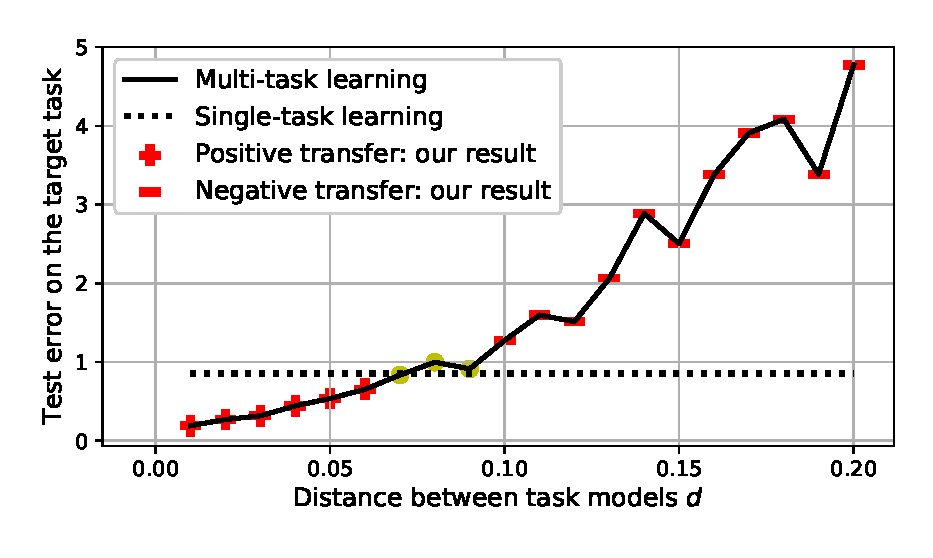
\includegraphics[width=0.5\textwidth]{figures/model_shift_phase_transition.eps}
	\caption{Positive vs negative transfer as a parameter of the task model distances.}
	\label{fig_model_shift_phasetrans}
\end{figure}









\subsection{Gains of Transfer Learning over Single-Task Training}

%\subsubsection{Gains over Single-Task Training}

\paragraph{A precise bound when there is no model shift.}
As Proposition \ref{prop_monotone} shows, if $\beta_s$ and $\beta_t$ are equal, then adding the source task dataset always helps learn the target task.
The goal of this section is to understand how covariate shift affects the rate of transfer. \todo{add conceptual msg}

%The key quantity is to look at:
%The estimator using the source and target together from minimizing \eqref{eq_mtl_basic} is
%\[ \hat{\beta}_{s,t} = (X_1^{\top} X_1 + X_2^{\top} X_2)^{-1} (X_1^{\top}Y_1 + X_2^{\top}Y_2)\]
%The estimation error of $\hat{\beta}_{s,t}$ is
%\begin{align}\label{eq_two_task}
%  \err(\hat{\beta}_{s,t}) = \sigma^2 \cdot \tr[(X_1^{\top}X_1 + X_2^{\top} X_2)^{-1}].
%\end{align}
%The estimation error using the target alone is
%\begin{align}\label{eq_target_task}
%	\err(\hat{\beta}_t) = \sigma^2 \cdot \tr[(X_2^{\top} X_2)^{-1}].
%\end{align}
%The improvement of estimation error from adding the source task is then given by
%$\err(\hat{\beta}_t) - \err(\hat{\beta}_{s,t})$.
%For the test error on the target task, the improvement from adding the source task is
%\[ \te(\hat{\beta}_t) - \te(\hat{\beta}_{s,t}) = \sigma^2\cdot\bigtr{\bigbrace{(X_2^{\top}X_2)^{-1} - (X_1^{\top}X_1 + X_2^{\top}X_2)^{-1}}\cdot\Sigma_2}. \]

%We calculate the amount of improvement by comparing equation \eqref{eq_two_task} to equation \eqref{eq_target_task}.
A simple observation here is that when $\beta_s = \beta_t$, the optimal $\hat{w}$ for minimizing equation \eqref{eq_te_mtl} is equal to $1$.
Based on this observation, we can get a more precise result than Theorem \ref{thm_model_shift} on the improvement of adding the source task data that only depends on the covariance matrices $\Sigma_1, \Sigma_2$ and the number of data points $n_1, n_2$.

\begin{proposition}[Transfer rate without model shift]\label{thm_cov_shift}
	When $\beta_s = \beta_t$, we have that the optimal ratio for $W_1/W_2$ in equation \eqref{eq_te_mtl} is $\hat{w} = 1 \pm \bigo{\frac 1 {n_1+n_2}}$ \todo{(figure out the constants)}.
	And
	\begin{align*}
		%\err(\hat{\beta}^{\TL}_{s,t}) &= \sigma^2 \cdot \bigtr{\frac 1 {(n_1 + n_2)a_1\Sigma_1 + (n_1 + n_2)a_2\Sigma_2}} \\
		\te(\hat{\beta}^{\TL}_{t}) &= \sigma^2 \cdot \bigtr{\bigbrace{(n_1 + n_2)a_1\Sigma_2^{-1/2}\Sigma_1\Sigma_2^{-1/2} + (n_1 + n_2)a_2\id}^{-1}} + \bigo{\frac 1 {(n_1 + n_2)^2}},
	\end{align*}
	where $a_1, a_2$ are the solutions of equations \eqref{eq_a2}.
\end{proposition}

As a remark, we see that Proposition \ref{prop_monotone} follows from Theorem \ref{thm_cov_shift}.
The amount of reduction on test error for the target task is given as
	\begin{align*}
%		\err(\hat{\beta}_t) - \err(\hat{\beta}_{s,t})
%		&= \sigma^2 p \cdot \bigtr{\frac 1 {(n_2 - p) \Sigma_2} - \frac 1 {(n_1 + n_2)a_1 \Sigma_1 + (n_1 + n_2)a_2 \Sigma_2}}, \\
		\te(\hat{\beta}_t) - \te(\hat{\beta}_{s,t})
		&= \sigma^2 \cdot \bigbrace{\frac p {n_2 - p} -  \bigtr{\bigbrace{(n_1 + n_2)a_1\Sigma_2^{-1/2}\Sigma_1\Sigma_2^{-1/2} + (n_1 + n_2)a_2\id}^{-1}}}.
	\end{align*}
Because
\begin{align*}
	\te(\hat{\beta}_{s,t}) \le \te(\hat{\beta}_t)
	\Leftarrow~ & (n_2 - p)\Sigma_2 \preceq (n_1 + n_2) a_1 \Sigma_1 + (n_1 + n_2)a_2 \Sigma_2 \\
	\Leftrightarrow~ & \zeroMatrix \preceq (n_1 + n_2) a_1 \Sigma_1 + (n_1 - (n_1 + n_2)\cdot a_1) \Sigma_2,
\end{align*}
which is true since $a_1 \le n_1 / (n_1 + n_2)$ by equation \eqref{eq_a2}.
The proof for $\te(\hat{\beta}_{s,t}) \le \te(\hat{\beta}_t)$ follows by multiplying $\Sigma_2^{-1/2}$ on both sides of the inequalities above.

\medskip
Now we apply Theorem \ref{thm_cov_shift} to show how covariate shift affects the rate of transfer.

%\begin{example}[\textbf{When $\Sigma_1 = \Sigma_2$}]
%In this case, we have $\lambda_i = 1$ for all $1\le i\le p$.
%And $a_1 + a_2 = 1 - p / (n_1 + n_2)$.
%Hence
%\[ \te(\hat{\beta}_{s,t}) = \frac{\sigma^2 p^2}{n_1 + n_2 - p} \text{ and } \err(\hat{\beta}_{s,t}) = \frac {\sigma^2 p} {n_1 + n_2 - p} \bigtr{\Sigma_2^{-1}}. \]
%\end{example}

\smallskip
\begin{example}[\textbf{When $\Sigma_1 = \Sigma_2 / \lambda$}]
In this case, equations \eqref{eq_a2} become
\[ a_1 + a_2 = 1 - p/(n_1 + n_2), a_1 + \frac{p}{n_1 + n_2} \cdot \frac {a_1} {a_1 + \lambda^2 a_2} = \frac{n_1} {n_1 + n_2}. \]
By solving these, we can get the test errors (the estimation error behaves similarly).
Figure \ref{fig_te_scaling} shows how they grow as we increase the number of source task data points.
Here $n_2 = 4p$ and $n_1$ ranges from $p$ to $20p$.
We can see that the smaller $\lambda$ is, the lower the test errors will be.
\end{example}

\smallskip
\begin{example}[\textbf{When $\Sigma_1$ and $\Sigma_2$ are complementary}]
	We consider two cases when $\Sigma_1$ and $\Sigma_2$ are \textit{different}
\begin{itemize}
	\item {\bf Different singular values:} Here we have that for $\Sigma_1^{-1/2}\Sigma_2^{1/2}$, the first $p/2$ singular values of $\Sigma_1$ is $\lambda$ and the rest is $1/\lambda$.
For this case, equations \eqref{eq_a2} become
\[ a_1 + a_2 = 1 - \frac{p}{n_1 + n_2}, a_1 + \frac{p}{2(n_1 + n_2)}\cdot \bigbrace{\frac{a_1}{a_1 + \lambda^2 a_2} + \frac{a_1}{a_1 + \frac{a_2}{\lambda^2}}} = \frac{n_1}{n_1 + n_2}. \]
It's not hard to verify that there is only one valid solution from the above.
After solving these, we get the test error for the target task as follows.
\[ \frac{p}{2(n_1 + n_2)} \cdot \bigbrace{\frac{1}{\frac{a_1}{\lambda^2} + a_2} + \frac{1}{a_1\lambda^2 + a_2}}.\]
	\item {\bf Different singular spaces:}
	Suppose $\Sigma_1$ and $\Sigma_2$ have the eigendecomposition
$$\Sigma_1^{1/2} = 1+ U\Lambda U^\top, \quad \Sigma_2^{1/2} = 1+ V\Lambda V,$$
where
$$\Lambda = \diag(\wt\lambda_1,\cdots, \wt\lambda_{p/2}), \quad U= (u_1,\cdots, u_{p/2}), \quad V= (v_1,\cdots, v_{p/2}).$$
We consider two case: if $V=U$, then $M=\id;$ if $V=U_\perp$ (i.e. the space spanned by $V$ is perpendicular to that spanned by $U$), then
$$M=\Sigma_1^{1/2} \Sigma_2^{-1/2}=(1+\Lambda)UU^\top + (1+\Lambda)^{-1}V V^\top .$$
This is an extension of the above example of complementary case.
\end{itemize}
\end{example}



In Figure \ref{fig_te_complement}, we plot the test error of the target task for $n_2 = 4p$ and $n_1$ ranging from $p$ to $20p$.
We observe the following two phases as we increase $n_1 / p$.
\begin{itemize}
	\item When $n_1 \le n_2$, having complementary covariance matrices leads to lower test error compared to the case when $\Sigma_1 = \Sigma_2$.
	\item When $n_1 > n_2$, having complementary covariance matrices leads to higher test error compared to the case when $\Sigma_1 = \Sigma_2$.
\end{itemize}

\begin{figure}
	\centering
	\begin{minipage}{0.48\textwidth}
		\centering
		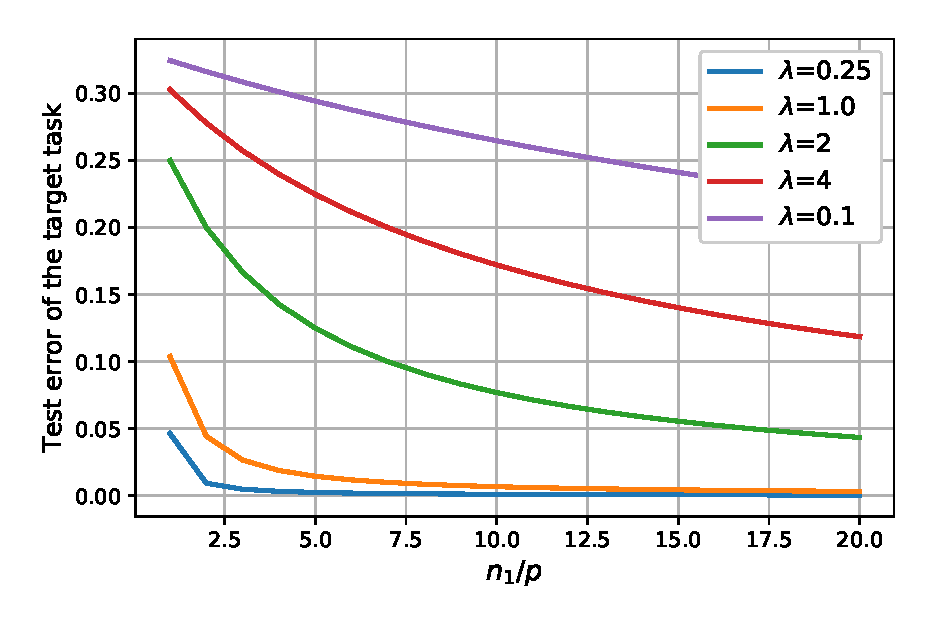
\includegraphics[width=0.9\textwidth]{figures/scaling.eps}
		\caption{When $\Sigma_1 = \Sigma_2 / \lambda$.}
		\label{fig_te_scaling}
	\end{minipage}\hfill
	\begin{minipage}{0.48\textwidth}
		\centering
		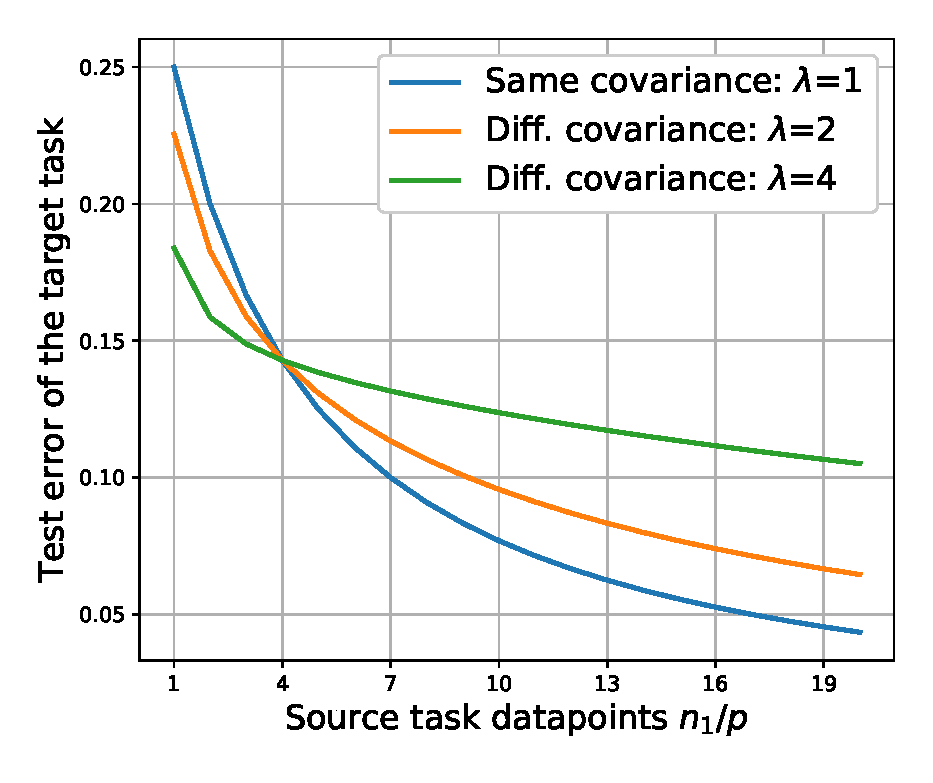
\includegraphics[width=0.9\textwidth]{figures/complementary.eps}
		\caption{When $\Sigma_1$ and $\Sigma_2$ are complementary. The number of target task data points is $n_2 = 4p$.}
		\label{fig_te_complement}
	\end{minipage}
\end{figure}


\paragraph{Extending the intuition to the general case.}
When there is model shift, i.e. $\beta_s = \beta_t$, we can still use Theorem \ref{thm_model_shift} (and Proposition \ref{prop_model_shift_tight}) to get the result.
\begin{itemize}
	\item \textbf{The effect of covariate shift:}
	\item \textbf{The effect of data ratio:}
\end{itemize}



\subsection{Gains of Transfer Learning over Multi-Task Training}



\section{The Case with Many Tasks of the Same Covariates}















